%\documentclass[12pt,convert={density=150}]{standalone}
\documentclass[12pt]{standalone}

\usepackage{amsmath}
\usepackage{amsfonts}
\usepackage{amssymb}
\usepackage{fontspec}
\usepackage{tikz}

\usetikzlibrary{arrows}
\usetikzlibrary{decorations.markings}
\usetikzlibrary{decorations.text}
\usetikzlibrary{matrix}
\usetikzlibrary{positioning}

\definecolor{myblue}{RGB}{38,120,179}

\begin{document}
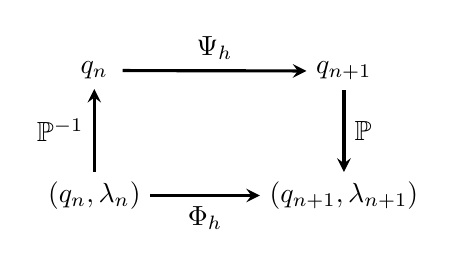
\begin{tikzpicture}[scale=2]
\matrix (m) [matrix of math nodes,row sep=3em,column sep=4em,minimum width=2em] {
q_{n} & q_{n+1} \\
(q_{n}, \lambda_{n}) & (q_{n+1}, \lambda_{n+1}) \\
};

\path[-stealth, line width=.4mm]
(m-1-1) edge node [above] {$\Psi_{h}$}       (m-1-2)
(m-2-1) edge node [left]  {$\mathbb{P}^{-1}$}   (m-1-1)
(m-1-2) edge node [right] {$\mathbb{P}$}        (m-2-2)
(m-2-1) edge node [below] {$\Phi_{h}$}       (m-2-2);
\end{tikzpicture}
\end{document}
